%%%%%%%%%%%%%%%%%%%%%%%%%%%%%%%%%%%%%%%%%%%%%%%%%%%%%%%%%%%%%%%%%%% 
%                                                                 %
%                           INLEIDING                             %
%                                                                 %
%%%%%%%%%%%%%%%%%%%%%%%%%%%%%%%%%%%%%%%%%%%%%%%%%%%%%%%%%%%%%%%%%%% 


\chapter{Testen en Resultaten}  

In dit hoofdstuk worden de resultaten van het programma besproken. Vooraleer dit gedaan wordt zal er gekeken worden hoe de add-on moet worden geïnstalleerd en gebruikt in Blender. Dit zal worden gedaan aan de hand van een stappenplan.
\par
Er worden ook enkele valkuilen besproken die er in de loop van dit onderzoek zijn opgedoken en hoe deze worden opgelost. Sommige van deze valkuilen vormen echter grote problemen die in Blender moeilijk of niet kunnen worden opgelost. Er zal vermeld worden hoe deze problemen in dit onderzoek zullen worden omzeild.
\par
Er zal in dit hoofdstuk ook een vergelijking worden gedaan tussen de kristalvisualisatiesoftware die op het moment van dit onderzoek gebruikt worden, en Blender als visualisatietool voor kristallen. Dit zal onder andere gedaan worden op basis van snelheid van het programma, gebruiksvriendelijkheid en uitbreidbaarheid.
\par
Net zoals in hoofdstuk vier zal er voornamelijk gebruik worden gemaakt van de actieve schrijfwijze en de wetenschappelijke 'we'-vorm. 


\section{Gebruiken van de add-on}
Deze sectie dient als een handleiding een gebruiker kan volgen om onze add-on te installeren in Blender en ze te gebruiken. Dit gaan we doen in de vorm van een stappenplan. 
\par
Dit is het stappenplan voor de installatie en het gebruik van de add-on op het besturingssysteem Windows. De add-on zou moeten werken op andere besturingssystemen maar de installatie van de add-on op deze gaan we niet bekijken. 

\subsection{Stap 1: Blender downloaden}
Als eerste moeten we Blender downloaden op ons syteem. Onze add-on is gemaakt voor versie 2.8x van Blender. In deze versie is er veel vernieuwd aan de Blender API waardoor de add-on niet achterwaarts compatibel is. Dit wil zeggen dat de add-on niet zal werken op oudere versies van Blender zonder de code aan te passen. In dit hoofdstuk spreken we, tenzij anders vermeld, altijd over de 2.8x versie van Blender .  
\par
Blender kan gedownload worden op de downloadpagina van hun offiële website:\url{https://builder.blender.org/download/}. Hier kiezen we het besturingssysteem en de bit-versie van ons systeem, en selecteren we de nieuwste versie van Blender, rode kader op Figuur[].  Dit download het ZIP-bestand waarin de Blender installatie staat. Als de download voltooid is kunnen we het ZIP-bestand uitpakken op ons systeem. Dit creëert een map waarin de Blender installatie staat. In deze map vinden we het uitvoerbare bestand \textit{blender.exe}, waarmee we Blender opstarten. Dit is tevens ook de map waarin we de CifFile module in plaatsen, zie eerste sectie van hoofdstuk vier.      

\begin{figure}[h]
\begin{center}
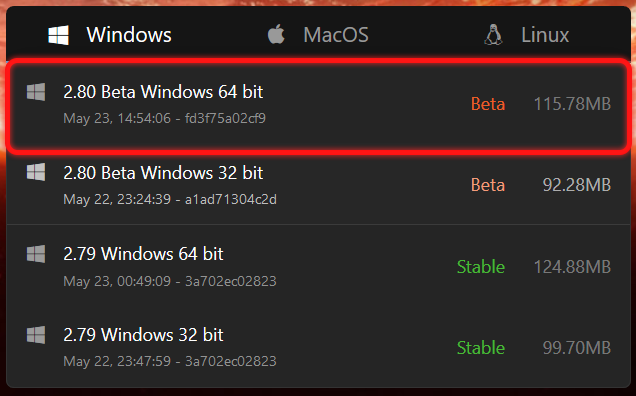
\includegraphics[scale=0.5]{b_download.png}
\caption{Overzicht van Blenderversies op downloadpagina van blender}
\end{center}
\end{figure}
 
\subsection{Stap 2: Externe programma's installeren}
Om de add-on te laten werken moeten we de OpenBabelGUI en de CifFile module van PyCIFRW op ons systeem installeren. We kunnen deze programma's downloaden op volgende webpagina's:
\begin{itemize}
\item OpenBabelGUI: \url{http://openbabel.org/wiki/Category:Installation}
\item PyCIFRW: \url{https://pypi.org/project/PyCifRW/#description}
\item CifFile map: \url{https://github.com/JarritB/Thesis/tree/master/} 
\end{itemize}   

Hoe we deze programma's werkende krijgen op ons systeem wordt uitgelegd in de eerste sectie van hoofdstuk vier. 
\par

\subsection{Stap 3: Add-on toevoegen}
We kunnen onze add-on downloaden vanop de GitHub pagina van dit onderzoek: 
   

  
\section{•}
Blender 2.80 is op het moment van dit onderzoek nog een beta versie, dit wil zeggen dat de versie instabiel zou kunnen zijn. Deze instabiliteit heeft echter geen problemen 
   